\documentclass[12pt]{article}

\usepackage[utf8]{inputenc}
\usepackage[brazil]{babel}
\usepackage[a4paper,left=3cm, right=2cm,top=2.5cm, bottom=2.5cm]{geometry}
\usepackage{amsmath}
\usepackage{graphicx}
\usepackage{float}
\usepackage{multirow}
\usepackage{authblk}
\usepackage{fancyhdr}
\usepackage{xcolor}
\usepackage{cite}


\title{\textbf{ENG1456 - Redes Neurais - Trabalho 2 Previsão de Séries Temorais}}
\author{\textbf{Aluno: Matheus Carneiro Nogueira - 1810764}}
\affil{}
\author{\textbf{Professora: Marley Velasco}}
\affil{}
\pagestyle{fancy}
\fancyhf{}
\lhead{{\small \textcolor{gray}{PUC-Rio ENG1456}}}
\renewcommand{\headrulewidth}{0pt}
\date{}
\renewcommand{\footrulewidth}{0pt}
\fancyfoot[C]{\thepage}

\begin{document}
	\maketitle
	\tableofcontents
	
	
	\begin{abstract}
		Este documento consiste no relatório do trabalho 2 do módulo de Redes Neurais da disciplina ENG1456 da PUC-Rio. Nele será explicada a implementação de modelos de Redes Neurais MLP para a previsão de uma série temporal do dataset MicroClima2 , disponibilizado pela professora da disciplina. A seções do relatório são definidas de acordo com as perguntas principais que constam no arquivo Guia de Atividades II. Foram consultados os materiais de aula, o livro \cite{livro} e outros materiais devidamente referenciados.
	\end{abstract}
		
	\section{Compreensão do Problema}
	\subsection{Visualize, em forma de gráfico, a dinâmica temporal da série escolhida. A série é adequada para a modelagem usando Redes Neurais? Caso não seja, que técnicas podem ser aplicadas para ajustar o comportamento da série?}\label{subsec:1.1}
	
	A série utilizada neste trabalho, denominada \textit{microclima2} consiste em 144 temperaturas média mensais, ou seja, temos informação sobre as temperaturas dos últimos 12 anos.
	
	Com o intuito de analisar a dinâmica temporal da série, foi gerado o gráfico da série em si e da decomposição dela, com o intuito de verificar \textit{trending} e \textit{sazonalidade}. As figuras abaixo ilustram esses resultados.
	
	\begin{figure}[H]
		\centering
		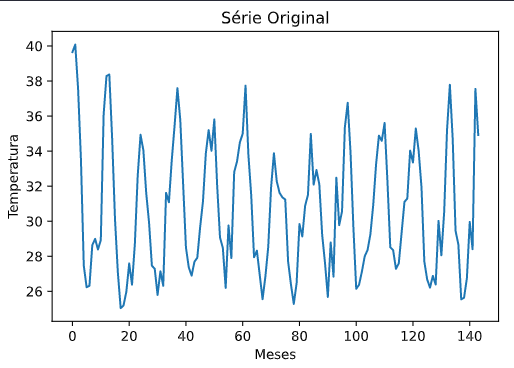
\includegraphics[width=0.7\linewidth]{Imagens/serieoriginal/plotserie}
		\caption{Série Original}
		\label{fig:plotserie}
	\end{figure}
	\begin{figure}[H]
		\centering
		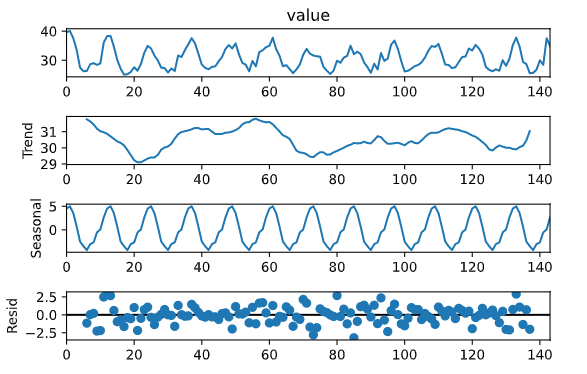
\includegraphics[width=0.7\linewidth]{Imagens/serieoriginal/decomposeSerie}
		\caption{Decomposição da Série Original}
		\label{fig:decomposeserie}
	\end{figure}

	Ao analisar a figura \ref{fig:plotserie} notamos que a série possui um perfil estacionário ao longo dos 12 anos. Isso quer dizer que a temperatura média de cada mês do ano \textit{a} é similar à temperatura média de cada mês no ano \textit{a+1}. Além disso, a figura \ref{fig:decomposeserie} revela, em seu campo \textit{Trend}, a tendência da série ao longo do tempo. Embora existam oscilações nesse gráfico, não se percebe nenhuma tendência geral da série. Com o intuito de ir além da análise visual, foi executado o \textit{Augmented Dickey-Fuller test} para verificar a probabilidade de existência de uma raiz unitária, que indicaria perfil não estacionário. O resultado é expresso na figura abaixo.
	\begin{figure}[H]
		\centering
		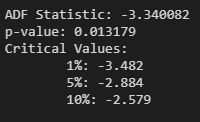
\includegraphics[width=0.5\linewidth]{Imagens/serieoriginal/asfteste}
		\caption{ADF Test}
		\label{fig:asfteste}
	\end{figure}
	
	Nota-se que o \textit{p-value} é muito pequeno e que o valor de \textit{ADF Statistic} é menor que o valor crítico para 1\%. Isso indica que esta série possui probabilidade baixíssima a alto grau de confiança em relação à inexistência de uma raiz unitária. Sendo assim, podemos tratá-la como uma série estacionária. Essa análise é importante pois, caso a série fosse não-estacionária, a rede neural precisaria, além de aprender o andamento temporal da série, aprender também a sua tendência, o que aumentaria a complexidade do modelo. Para corrigir esse problema, poderíamos tornar a série estacionária por meio de uma diferenciação, por exemplo, lembrando, apenas, de voltar aos valores originais ao final.
	
	Como a série em questão possui valores de temperaturas médias mensais ao longo dos anos, é de se esperar que exista uma sazonalidade razoavelmente perceptível. Ambas as figuras \ref{fig:plotserie} e \ref{fig:decomposeserie} mostram que essa sazonalidade existe de fato. Com essas imagens em mãos e supondo que o mês 1.0 é Janeiro, podemos inferir que as temperaturas referem-se a um local do hemisfério sul, onde é verão em janeiro, uma vez que as maiores temperaturas encontram-se próximas desse mês. Essa informação (o mês da temperatura) será útil para o treinamento da série, portanto deve constar nos dados de entrada. Como a sazonalidade não oferece problemas para a modelagem com um \textit{MLP}, não precisamos fazer nenhum tipo de correção.
	
	
	\subsection{No problema escolhido, usaremos uma variável exógena que representa	o mês de previsão (i.e. no instante t+1). De que forma esta variável pode auxiliar na previsão da série temporal?}
	
	Como comentado na seção \ref{subsec:1.1}, a série de temperaturas apresenta sazonalidade anual, isto é, o perfil de evolução da séria se repete de ano em ano, o que é de se esperar dada a natureza da série. Desse modo, fornecer o mês do valor de entrada pode auxiliar bastante na qualidade da previsão da série, uma vez que meses como Dezembro a Fevereiro (12 a 3) geralmente apresentam temperaturas médias mais altas, enquanto meses como Maio a Setembro (5 a 9) apresentam temperaturas mais baixas. Ao fornecer essa informação para Rede Neural, ela possuirá mais informações para aprender o perfil de sazonalidade da série, aumentando sua qualidade de previsão. 
	
	\section{Previsão One-Step}
	
	\subsection{Execute o script para a previsão one-step. Analise o resultado (conjunto	de treinamento e teste), usando as métricas RMSE e MAE.}\label{subsec:2.1}
	
	Para realizar a previsão de um passo à frente, foram testadas diversas configurações de redes neurais, variando a quantidade de neurônios na camada escondida. Os erros \textit{RMSE} e \textit{MAE} de cada uma dessas configurações estão apresentados na tabela a seguir. Vale comentar que, no arquivo \textit{jupyter notebook} enviado junto deste relatório está presente apenas o modelo final escolhido. Além disso, o script definia a métrica \textit{MSE}, então,para obter a métrica desejada, \textit{RMSE} foi calculada a raiz quadrada da \textit{MSE} fornecida.
	
	\begin{table}[H]\label{tab:comparacaoNeuronios}
		\centering
		\begin{tabular}{|l|l|l|l|l|l|l|}
			\hline
			\# neurônios & 5     & 10    & 15    & 20    & 25    & 30    \\ \hline
			RMSE         & 3.007 & 2.871 & 3.022 & 2.584 & 2.598 & 2.936 \\ \hline
			MAE          & 2.090 & 2.105 & 2.434 & 1.938 & 1.968 & 2.343 \\ \hline
		\end{tabular}
	\caption{Comparação dos Erros para diferentes números de neurônios}
	\end{table}

	\begin{figure}[H]
		\centering
		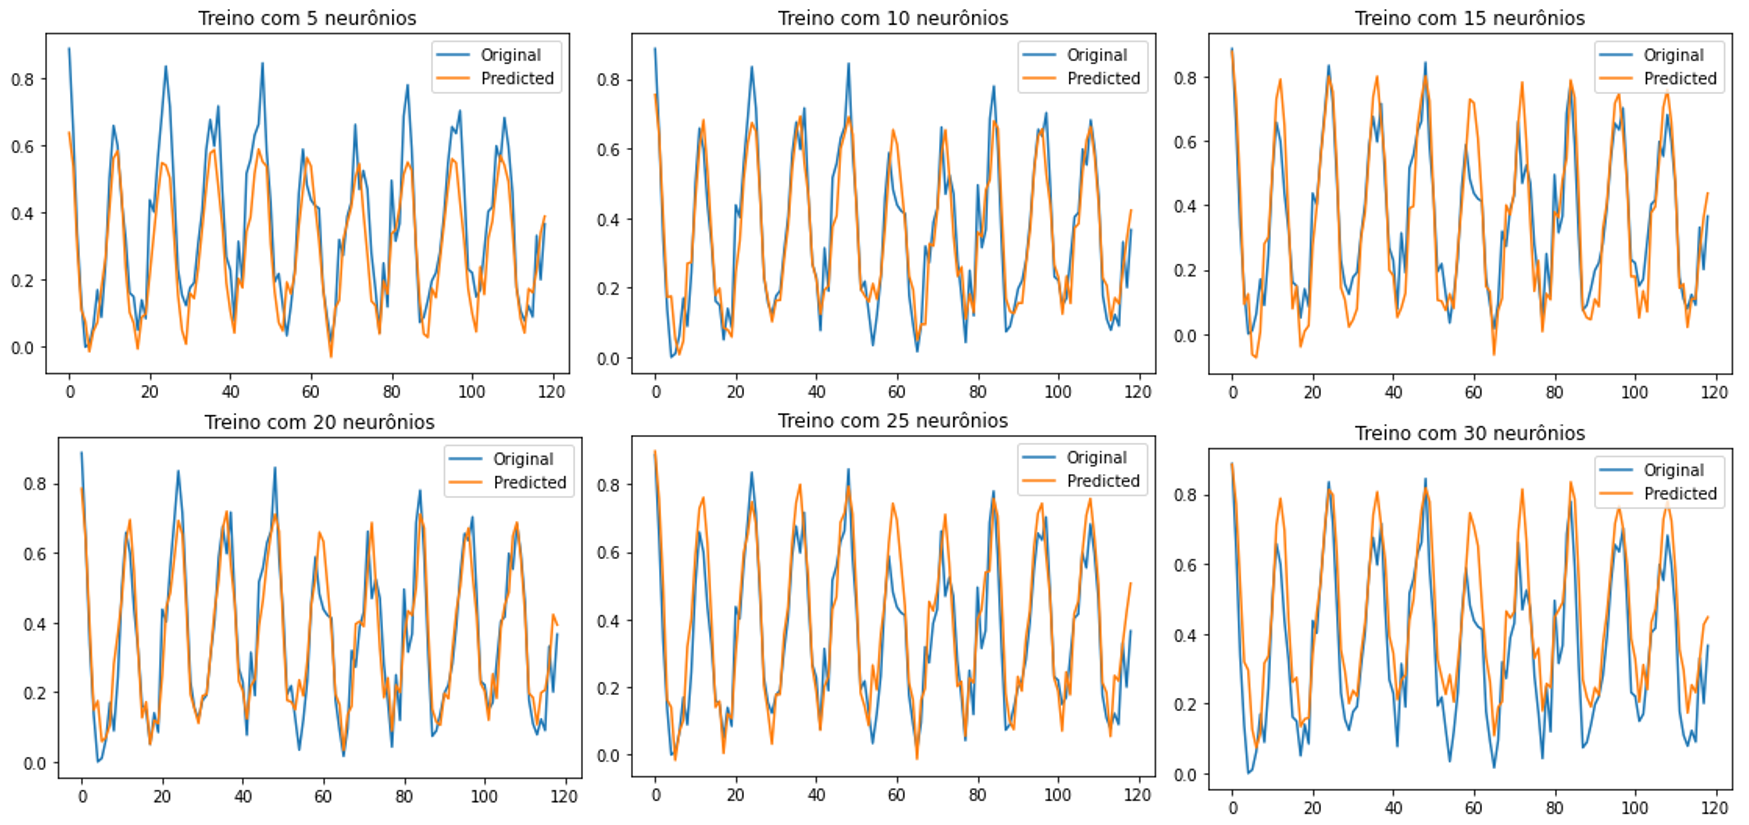
\includegraphics[width=0.9\linewidth]{Imagens/onestep/treinocomparadoneuronios}
		\caption{Comparação de Treinamento para diferentes quantidades de neurônios}
		\label{fig:treinocomparadoneuronios}
	\end{figure}
	\begin{figure}[H]
		\centering
		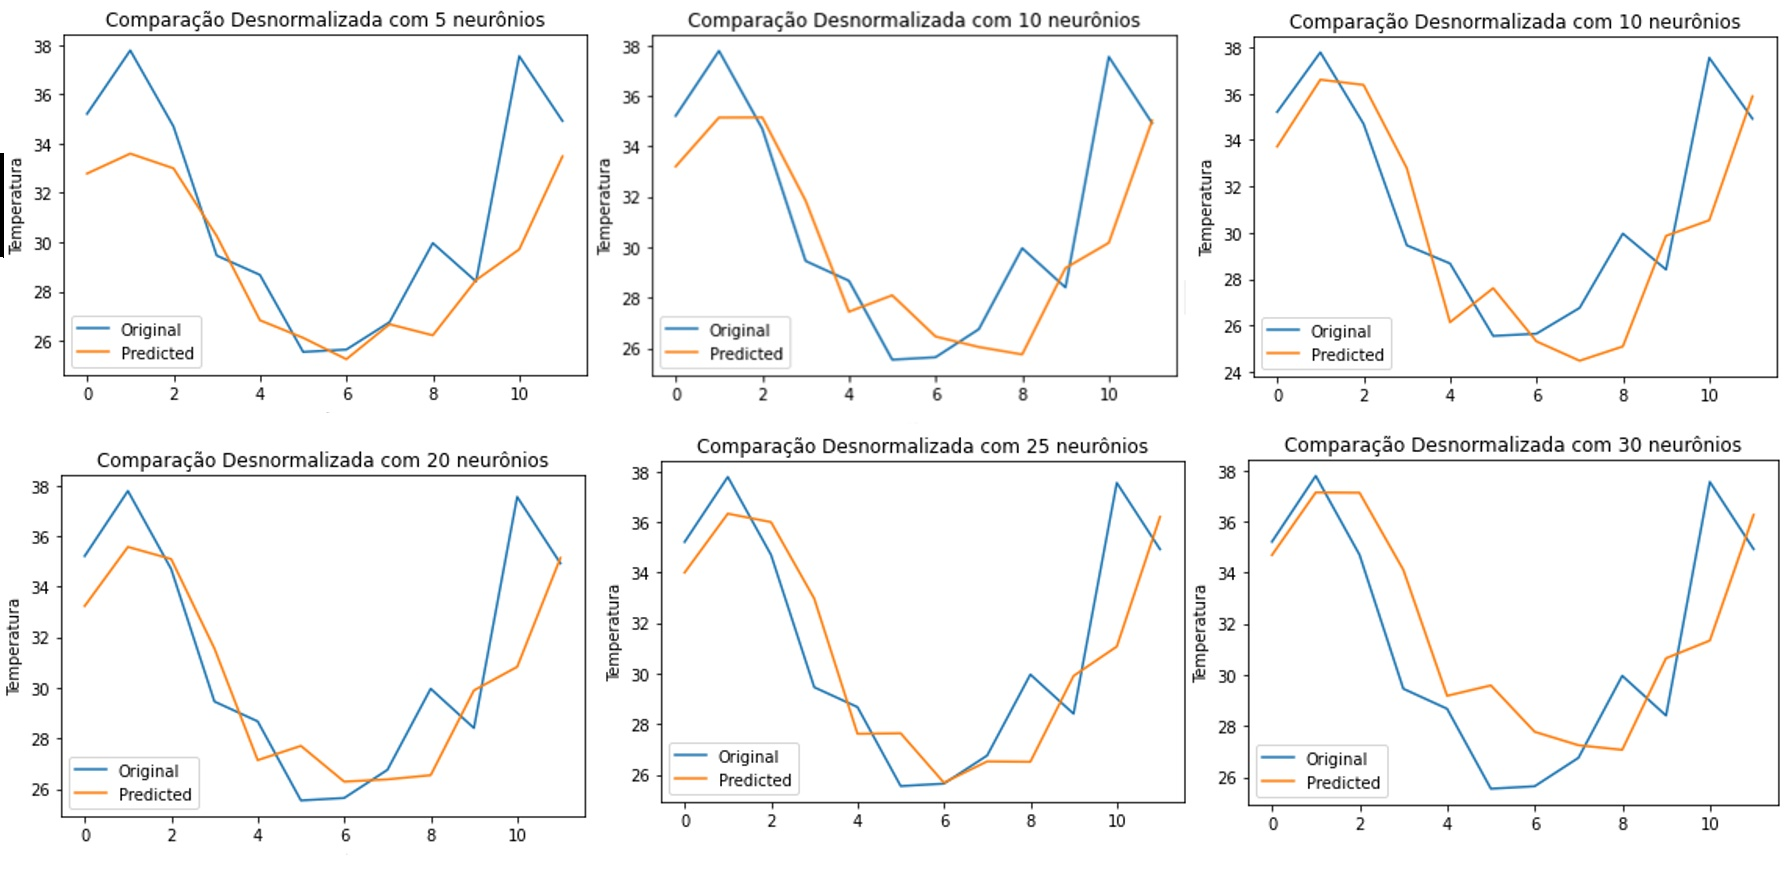
\includegraphics[width=0.9\linewidth]{Imagens/onestep/comparacaoneuronios.jpg}
		\caption{Comparação de testes para diferentes quantidades de neurônios}
		\label{fig:comparacaoneuronios}
	\end{figure}

	Com base na análise da tabela \ref{tab:comparacaoNeuronios} e das imagens \ref{fig:treinocomparadoneuronios} e \ref{fig:comparacaoneuronios}, percebe-se que para valores de 20 e 25 neurônios os erros são muito similares. Sendo assim, foi optado por eleger a rede com 20 neurônios na camada escondida por apresentar os melhores valores para as métricas analisadas e ser um modelo mais simples do que o de 25 neurônios.
	
	Podemos perceber perfeitamente, com as imagens acima, a importância da generalização e da especialização da rede. Note que para 5 neurônios a curva de treino e de teste é muito suave, o que indica que a rede não conseguiu aprender o suficiente por possuir poucos pesos treináveis. Ou seja, não adquiriu especialização. Por outro lado, com 30 neurônio a curva passa a ser desnecessariamente ruidosa devido à quantidade grande de parâmetros treináveis, causando perda de generalização.
	
	A figura abaixo exibe as métricas da rede escolhida.
	
	\begin{figure}[H]
		\centering
		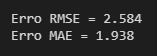
\includegraphics[width=0.4\linewidth]{Imagens/onestep/erros20}
		\caption{Erros da Rede Neural escolhida com 20 neurônios}
		\label{fig:erros20}
	\end{figure}
	
	
	
	\subsection{Modifique a técnica de codificação mensal de ‘numérico’ para ‘binário’. Qual a mudança existente na arquitetura da Rede Neural? Analise o resultado (conjunto de treinamento e teste), usando as métricas RMSE e MAE.}
	
	As redes treinadas até então já estavam com a codificação mensal binária. Sendo assim, foi criado um modelo com exatamente os mesmos parâmetros da rede escolhida na seção \ref{subsec:2.1} mas com a codificação numérica para os meses. Ao treinar essa nova rede pela primeira vez, os valores para as métrica \textit{RMSE} e \textit{MAE} foram melhores que aqueles apresentados pela rede com codificação binária. Para ter maior certeza dessa melhora, foram treinadas 6 redes com as mesmas configurações, variando, obviamente, apenas os pesos iniciais ,que são aleatórios. Os erros para as 6 redes encontram-se an tabela abaixo. A primeira coluna é a referência da rede com configuração binária.
	
	\begin{table}[H]\label{tab:binnum}
		\begin{tabular}{|l|l|l|l|l|l|l|l|}
			\hline
			\#Rede & Binária & 1     & 2     & 3     & 4     & 5     & 6     \\ \hline
			RMSE   & 2.584   & 2.448 & 2.276 & 2.572 & 2.386 & 2.587 & 2.827 \\ \hline
			MAE    & 1.938   & 1.751 & 1.741 & 1.910 & 1.842 & 1.871 & 2.104 \\ \hline
		\end{tabular}
		\centering
		\caption{Comparação dos erros das redes com codificação binária e numérica}
	\end{table}
	
	Ao analisar a tabela \ref{tab:binnum}, não é possível perceber grande melhora, ou piora, no desempenho da rede neural em relação ao tipo de codificação utilizado. Tentemos encontrar uma explicação para essa consistência. 
	
	Como visto na seção \ref{subsec:1.1}, a série em questão é bem comportada, inclusive em relação ao padrão de sazonalidade. O fato do tipo de codificação da entrada "mês" mão ter influenciado na qualidade da previsão pode ser explicado, justamente, por esse bom comportamento. Independente do tipo de codificação a Rede parece já possuir informações suficientes para fazer a previsão com uma boa qualidade. Além disso, o tipo de codificação também altera a quantidade de entradas da rede neural. No caso numérico há apenas 1 entrada para indicar o mês, enquanto no caso binário são 4 entradas. Essa diferença aumenta o número de pesos a serem treinados e aumenta a complexidade da rede, podendo gerar perda de generalização. No entanto, uma vez que as métricas obtidas não foram muito distintas, isso não ocorreu.
	
	Para as demais seções, foi utilizada a codificação numérica.
	
	\section{Previsão Multi-Step}
	
	\subsection{Implemente o processo de previsão multi-step}\label{subsec:multi1}
	
	A ideia central da previsão multi-step consiste em utilizar, ao invés de valores reais, valores previstos pela rede para "realimentar" a série. Em detalhes, para prever o valor da série em $t+1$, sabendo que utilizamos um \textit{lag} de 12 passos passados, precisamos fornecer os valores de $t-0$ até $t-11$ (além de outras possíveis variáveis externas, como o mês). Agora, para prever o valor da série em $t+2$, precisamos ainda fornecer 12 valores passados, mas sabendo que, desses, apenas 11 valores são reais, enquanto um é previsto. Isso quer dizer que, para prever $t+2$, precisamos fornecer $\bf{t+1}$ até $t-10$, sendo $t+1$ fruto de uma previsão. Com o intuito de prever 12 passos à frente, repetimos este processo até $t+12$.
	
	Para implementar essa previsão, foi desenvolvida a seguinte função:
	\begin{figure}[H]
		\centering
		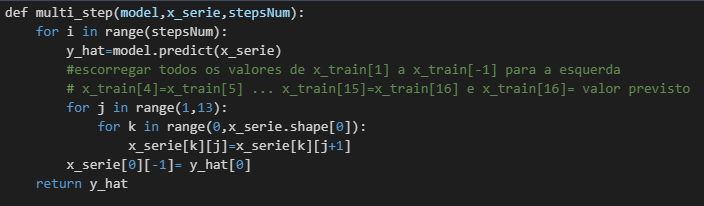
\includegraphics[width=0.7\linewidth]{Imagens/multistep/defmultistep}
		\caption{Função para a previsão multi-step}
		\label{fig:defmultistep}
	\end{figure}
	
	
	\subsection{Faça a previsão multi-step para o horizonte de previsão igual a 12 e compare com o resultado da previsão one-step.}
	
	Foi executada a função descrita anteriormente tanto para comparação com o conjunto de treino quanto para o conjunto de teste. As imagens abaixo ilustram essas execuções e a tabela, as métrica \textit{RMSE} e \textit{MAE}:
	\begin{figure}[H]
		\centering
		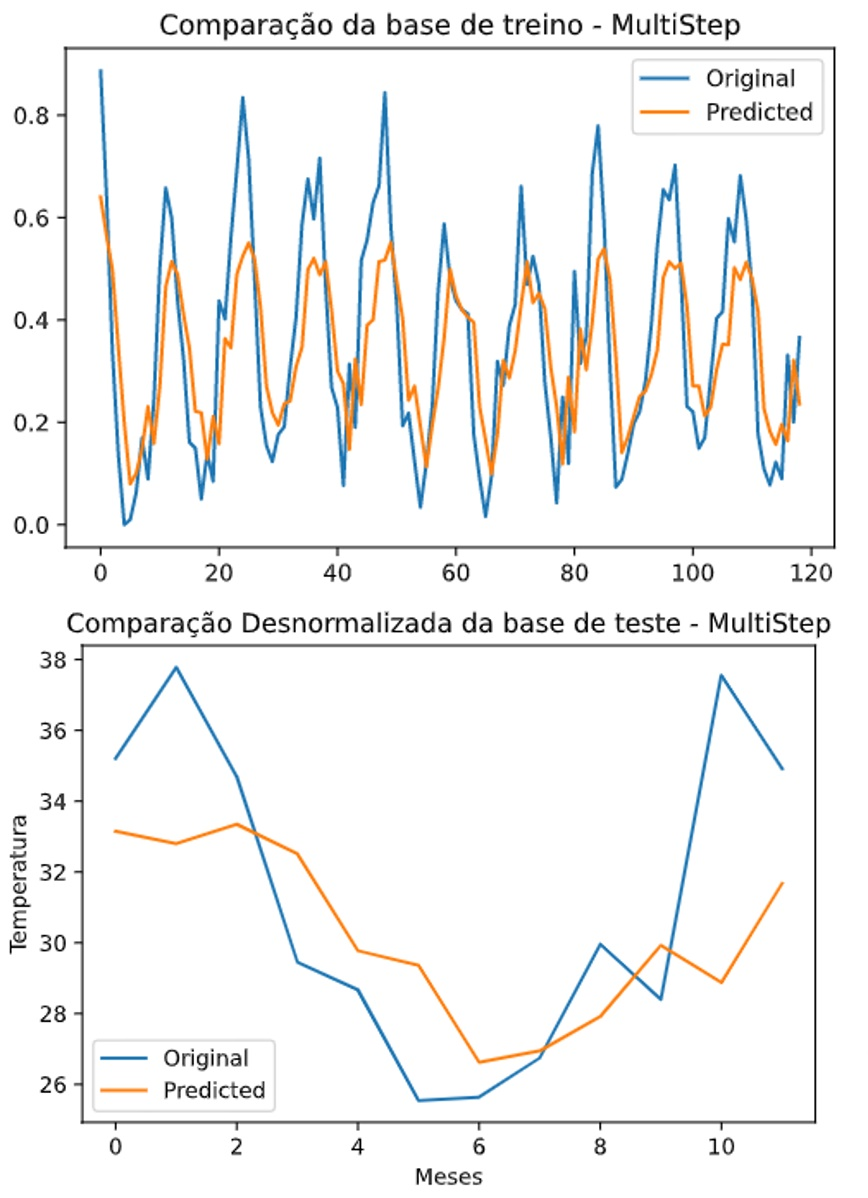
\includegraphics[width=0.7\linewidth]{Imagens/multistep/compMulti.jpg}
		\caption{Execução da Previsão Multi-Step}
		\label{fig:compmulti}
	\end{figure}
	\begin{table}[H]\label{tab:multiErros}
		\begin{tabular}{|l|l|l|}
			\hline
			\#Rede & Multi-Step & One-Step \\ \hline
			RMSE   & 3.528    & 2.584 \\ \hline
			MAE    &  2.753   & 1.938  \\ \hline
		\end{tabular}
		\centering
		\caption{Erros para a previsão multi step}
	\end{table}

	Pode-se perceber que o resultado da previsão multi-step foi consideravelmente pior que o da one-step. Um motivo que pode explicar essa piora, é o fato da previsão multi-step funcionar com a previsão de valores futuros com base em dados previstos, não apenas reais. Isso faz com que ocorra uma acumulação de erros ao longo da previsão. Sendo assim, não é de se estranhar que, embora entre os meses 2 e 9 os valores previstos e reais sejam similares, como mostra a figura \ref{fig:compmulti}, a previsão para os 3 últimos meses seja ruim. Outra característica que vale ser comentada é o perfil mais suave dos valores previstos em relação aos valores reais. Nota-se, também pela figura \ref{fig:compmulti}, que os valores previstos para o treinamento nunca alcançam a temperatura máxima nem a mínima.
	
	Dito isso, ainda existe a possibilidade de a perda de qualidade observada ser fruto da má implementação da previsão multi-step. Embora a lógica explicada na seção \ref{subsec:multi1} esteja correta, erros de programação podem ter sido cometidos. 
	
	Ao longo das próximas seções serão variados parâmetros da rede para tentar melhorar seu desempenho.
	
	
	\subsection{Modifique o tamanho da janela de entrada e avalie os resultados}
	
	Primeiramente, é necessário apontar que todas as janelas testadas são sequenciais, uma vez que a função de transformação de dados fornecida gera apenas janelas deste tipo. Ao modificar o tamanho da janela de entrada, o que estamos, de fato, fazendo, é alterando a quantidade de meses passados que a rede terá conhecimento para prever a temperatura do próximo mês. Não necessariamente fornecer mais meses para a rede influenciará positivamente a precisão. Como a série em questão é de temperaturas de um dado local, e apresenta um perfil sazonal forte, eventualmente fornecer apenas os últimos 6 meses, ou 4 meses seria o suficiente para a rede aprender o padrão de temperaturas. Uma possível melhor escolha de janela seria fornecer o último trimestre ou quadrimestre e a temperatura do mesmo mês da previsão, mas de um ano antes. No entanto, esta janela não foi testada por motivos já explicados.
	
	Outra influência do tamanho da janela é o dilema entre especialização e generalização. Como sabemos, maior janela equivale a mais dados de entrada que, por sua vez, equivale a mais pesos treináveis, maior complexidade da rede que pode levar a uma hiper especialização e perda de generalização. O raciocínio contrário também vale, menor janela, menos entradas, menos pesos, rede mais simples e risco de falta de especialização.
	
	Vejamos os resultados obtidos para os valores de janelas abaixo:
	
	\begin{table}[H]
		\centering
		\begin{tabular}{|l|l|l|l|l|l|l|l|}
			
			\hline
			\#Janela & 12    & 10    & 8     & 6     & 4     & 2     & 1     \\ \hline
			RMSE     & 2.584 & 2.906 & 2.873 & 2.557 & 2.546 & 3.359 & 2.854 \\ \hline
			MAE      & 1.938 & 2.238 & 2.305 & 2.007 & 1.926 & 2.73  & 1.975 \\ \hline
		\end{tabular}
		\caption{Erros para redes de diferentes tamanhos de janela}
	\end{table}

	\begin{figure}[H]
		\centering
		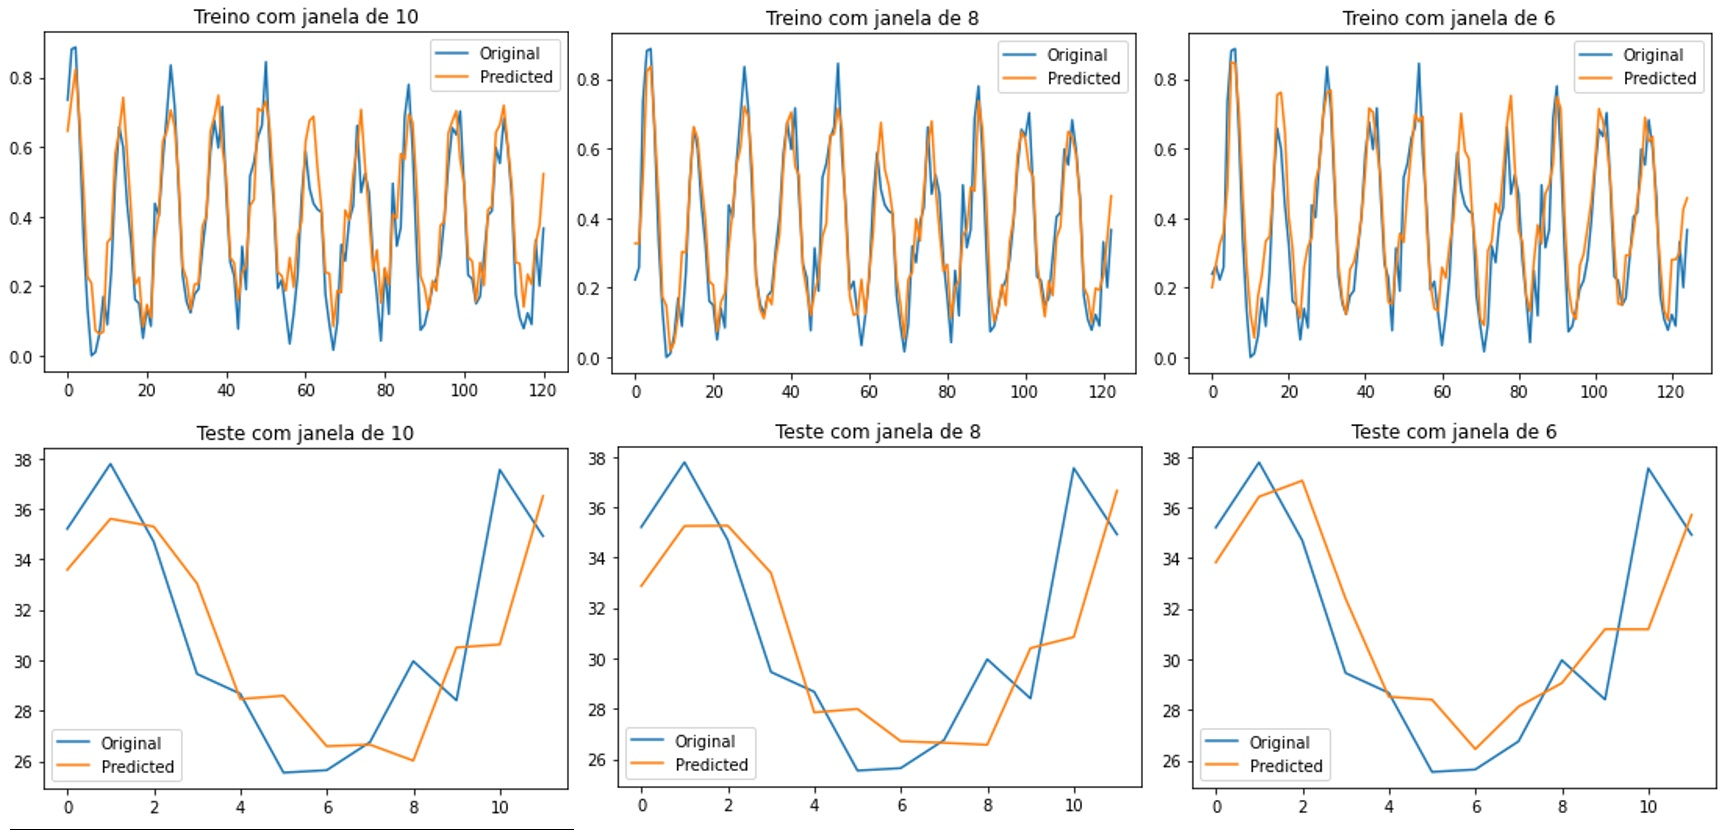
\includegraphics[width=0.9\linewidth]{Imagens/janelas/janelas6a10.jpg}
		\caption{Comparações de treino e teste para janelas 10, 8 e 6}
		\label{fig:janelas6a10}
	\end{figure}

	\begin{figure}[H]
		\centering
		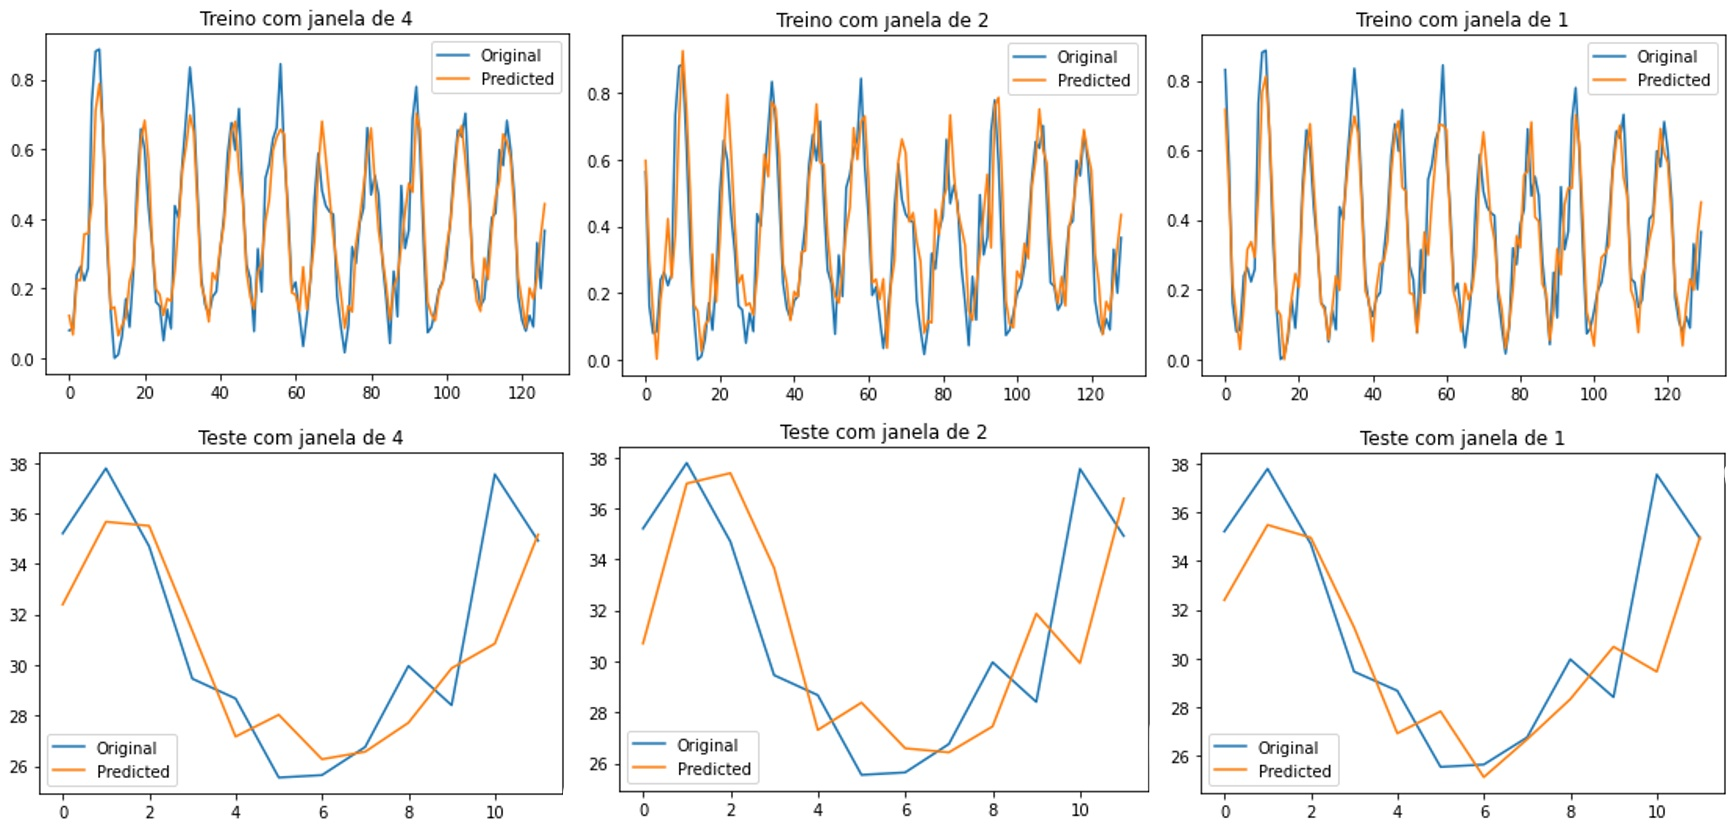
\includegraphics[width=0.9\linewidth]{Imagens/janelas/janelas1a4.jpg}
		\caption{Comparações de treino e teste para janelas 4, 2 e 1}
		\label{fig:janelas1a4}
	\end{figure}
	
	Percebe-se que os melhores resultados em termos dos erros analisados são para 12, 6 e 4 janelas. Assim como havíamos suposto e comentado, conhecer apenas o trimestre ou semestre passado, dada a sazonalidade e bom comportamento da série, mostra-se tão bom quanto conhecer o ano anterior inteiro. Sendo assim, como redes mais simples tendem a ser mais interessantes, a rede com janela de 4 meses seria a melhor escolha dentre as apresentadas.
	
	\subsection{Modifique a topologia da rede para obter um melhor desempenho. Altere seus parâmetros (e.g. número de processadores na camada escondida, tipo de função na camada de saída) e avalie o desempenho em termos das métricas RMSE e MAE.}
	
	\subsection{Implemente a codificação ‘1 of N’ e use-a para modificar a representação da variável ‘mês’. Qual a mudança existente na arquitetura da Rede	Neural? Avalie o desempenho em termos das métricas RMSE e MAE.}
	

	\bibliography{bibliografia} 
	\bibliographystyle{plain}
\end{document}